\subsubsection{Adams-Moulton}

Table \ref{tab:oscillation_errors_am} summarizes the Adams-Moulton error analysis. The implicit Adams-Moulton solvers behave much like the Adams-Bashforth-Moulton ones: they have similar errors and observed orders for the same formal order considered. However, the implicit Adams-Moulton class uses one less step with respect the corresponding Adams-Bashforth-Moulton class: this could lead to the promise of higher computational efficiency. Notwithstanding, for solving the implicit non-linearity embedded into the Adams-Moulton solvers an iterative algorithm must be employed: for the results presented, a 5 iterations of \emph{fixed point algorithm} have been computed. This strongly reduces the eventual gain of computational efficiency with respect the Adams-Bashforth-Moulton class.

\begin{table}[!ht]
  \centering
  \caption{Oscillation test: errors analysis of explicit Adams-Moulton solvers; the implicit non-linearity is solved by 5 iterations of \emph{fixed point algorithm}}\label{tab:oscillation_errors_am}
  \begin{subtable}[b]{0.40\textwidth}
    \centering
    \caption{1 step}\label{tab:oscillation-am-1}
    \resizebox{1.00\textwidth}{!}{%
    \begin{tabular}{ccccc}
      \toprule
      {\sc Time Step} & {\sc Error X} & {\sc Error Y} & {\sc Order X} & {\sc Order Y} \\
      \hline
      5000.0          &  0.840E+10    &  0.706E+10    & /             & /             \\
      2500.0          &  0.503E+06    &  0.570E+06    & 14.03         & 13.60         \\
      1250.0          &  0.289E+04    &  0.272E+04    &  7.45         &  7.71         \\
       625.0          &  0.239E+03    &  0.232E+03    &  3.59         &  3.55         \\
       320.0          &  0.737E+02    &  0.722E+02    &  1.76         &  1.74         \\
       100.0          &  0.250E+02    &  0.247E+02    &  0.93         &  0.92         \\
      \bottomrule
    \end{tabular}}
  \end{subtable}\quad%
  \begin{subtable}[b]{0.40\textwidth}
    \centering
    \caption{2 steps}\label{tab:oscillation-am-2}
    \resizebox{1.00\textwidth}{!}{%
    \begin{tabular}{ccccc}
      \toprule
      {\sc Time Step} & {\sc Error X} & {\sc Error Y} & {\sc Order X} & {\sc Order Y} \\
      \hline
      5000.0          &  0.108E+02    &  0.109E+02    & /             & /             \\
      2500.0          &  0.412E+01    &  0.419E+01    & 1.39          & 1.38          \\
      1250.0          &  0.148E+01    &  0.150E+01    & 1.48          & 1.48          \\
       625.0          &  0.527E+00    &  0.533E+00    & 1.49          & 1.49          \\
       320.0          &  0.193E+00    &  0.196E+00    & 1.50          & 1.50          \\
       100.0          &  0.338E-01    &  0.342E-01    & 1.50          & 1.50          \\
      \bottomrule
    \end{tabular}}
  \end{subtable}\\
  \begin{subtable}[b]{0.40\textwidth}
    \centering
    \caption{3 steps}\label{tab:oscillation-am-3}
    \resizebox{1.00\textwidth}{!}{%
    \begin{tabular}{ccccc}
      \toprule
      {\sc Time Step} & {\sc Error X} & {\sc Error Y} & {\sc Order X} & {\sc Order Y} \\
      \hline
      5000.0          &  0.390E+01    &  0.384E+01    & /             & /             \\
      2500.0          &  0.551E+00    &  0.544E+00    & 2.82          & 2.82          \\
      1250.0          &  0.947E-01    &  0.934E-01    & 2.54          & 2.54          \\
       625.0          &  0.167E-01    &  0.165E-01    & 2.50          & 2.50          \\
       320.0          &  0.313E-02    &  0.309E-02    & 2.50          & 2.50          \\
       100.0          &  0.171E-03    &  0.169E-03    & 2.50          & 2.50          \\
      \bottomrule
    \end{tabular}}
  \end{subtable}\quad%
  \begin{subtable}[b]{0.40\textwidth}
    \centering
    \caption{4 steps}\label{tab:oscillation-am-4}
    \resizebox{1.00\textwidth}{!}{%
    \begin{tabular}{ccccc}
      \toprule
      {\sc Time Step} & {\sc Error X} & {\sc Error Y} & {\sc Order X} & {\sc Order Y} \\
      \hline
      5000.0          &  0.983E+00    &  0.999E+00    & /             & /             \\
      2500.0          &  0.832E-01    &  0.845E-01    & 3.56          & 3.56          \\
      1250.0          &  0.736E-02    &  0.746E-02    & 3.50          & 3.50          \\
       625.0          &  0.652E-03    &  0.660E-03    & 3.50          & 3.50          \\
       320.0          &  0.626E-04    &  0.635E-04    & 3.50          & 3.50          \\
       100.0          &  0.107E-05    &  0.108E-05    & 3.50          & 3.50          \\
      \bottomrule
    \end{tabular}}
  \end{subtable}\\
\end{table}

Figure \ref{fig:results-oscillation-adams-moulton} shows similar plots of figure \ref{fig:results-oscillation-adams-bashforth-moulton} above discussed: there are not relevant differences between the 2 classes of solvers.

\begin{figure}[!ht]
  \centering
  \begin{subfigure}[b]{0.45\textwidth}
    \centering
    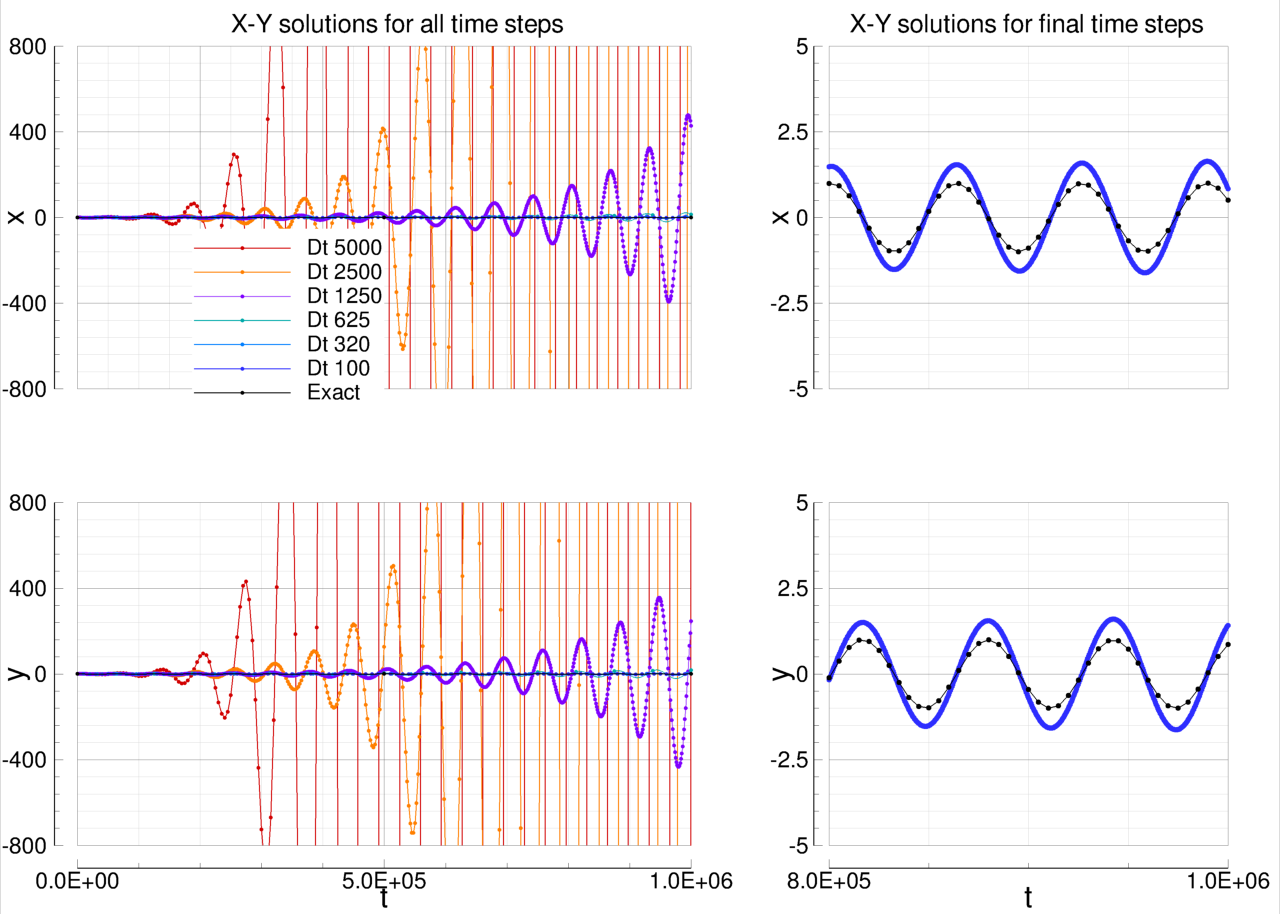
\includegraphics[width=1.00\textwidth]{errors-analysis/oscillation/errors_analysis-oscillation-adams-moulton-0.png}
    \caption{0 step}\label{fig:results-oscillation-adams-moulton-0}
  \end{subfigure}\quad%
  \begin{subfigure}[b]{0.45\textwidth}
    \centering
    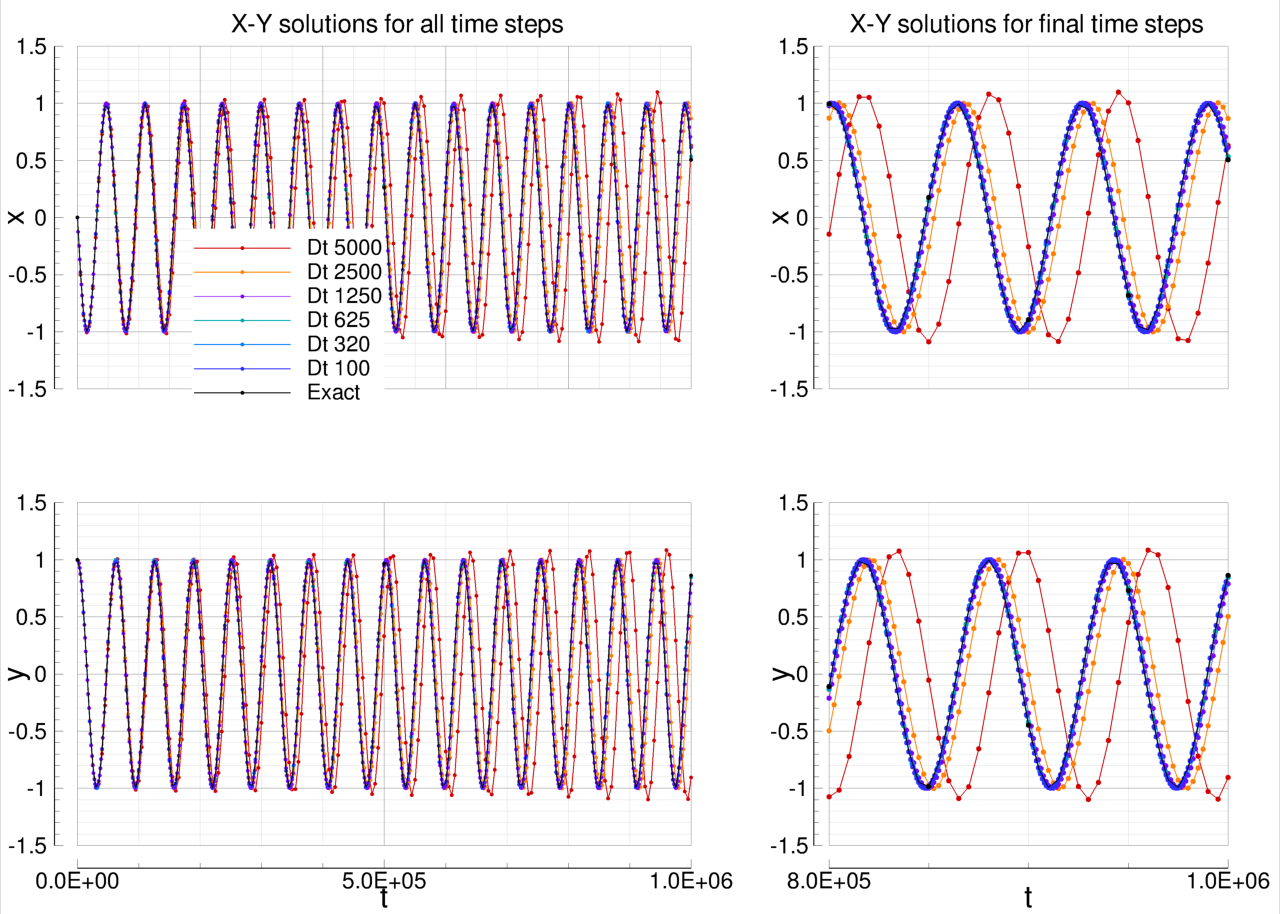
\includegraphics[width=1.00\textwidth]{errors-analysis/oscillation/errors_analysis-oscillation-adams-moulton-1.png}
    \caption{1 step}\label{fig:results-oscillation-adams-moulton-1}
  \end{subfigure}\\
  \begin{subfigure}[b]{0.45\textwidth}
    \centering
    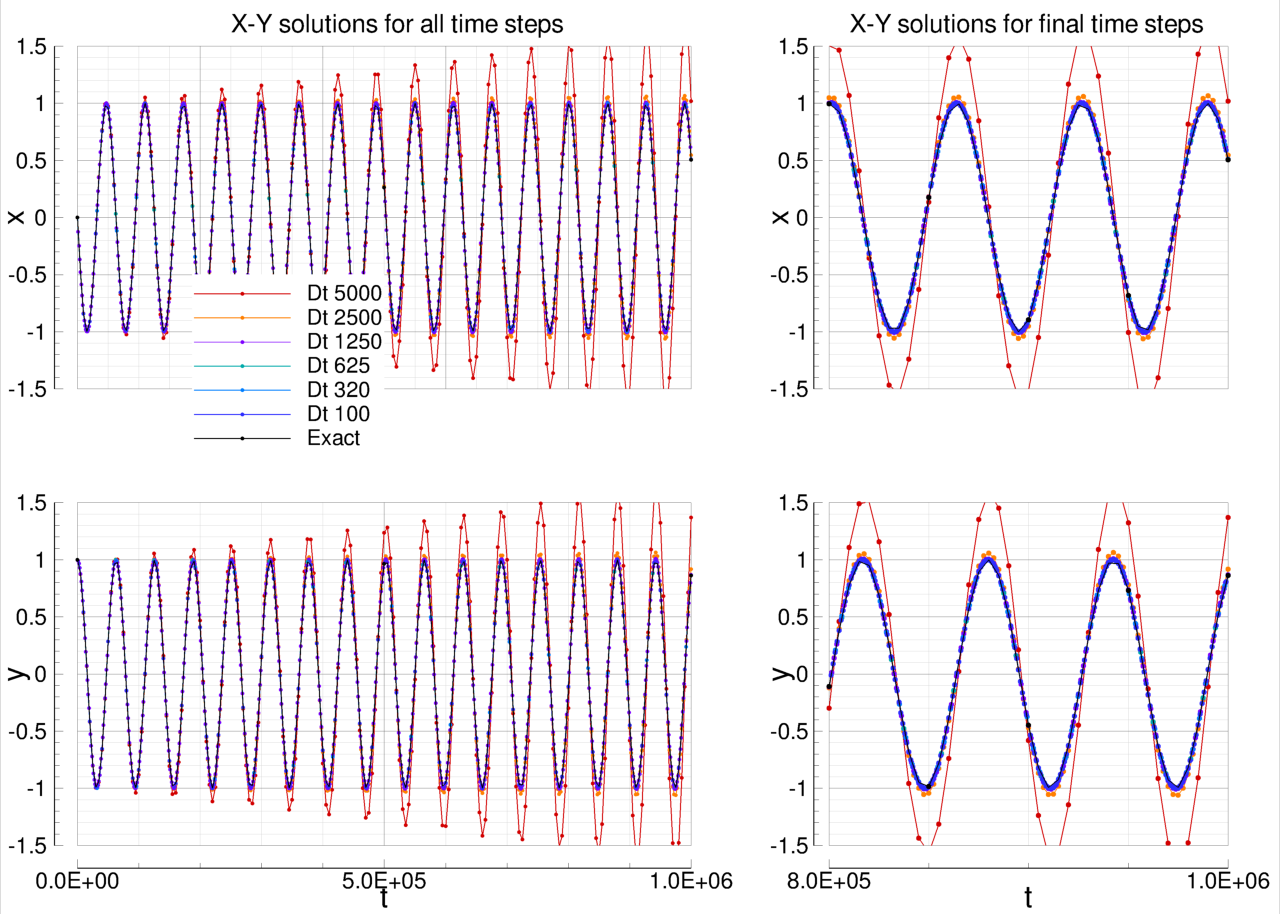
\includegraphics[width=1.00\textwidth]{errors-analysis/oscillation/errors_analysis-oscillation-adams-moulton-2.png}
    \caption{2 steps}\label{fig:results-oscillation-adams-moulton-2}
  \end{subfigure}\quad%
  \begin{subfigure}[b]{0.45\textwidth}
    \centering
    \includegraphics[width=1.00\textwidth]{errors-analysis/oscillation/errors_analysis-oscillation-adams-moulton-3.png}
    \caption{3 steps}\label{fig:results-oscillation-adams-moulton-3}
  \end{subfigure}
  \caption{Oscillation equations solutions computed by means of Adams-Moulton solvers}\label{fig:results-oscillation-adams-moulton}
\end{figure}

